\chapter{Sufixový strom}\label{chap:sx}

\emph{Sufixový strom} je písmenkový strom pre všetky \emph{sufixy (prípony)} 
daného slova. Jeho veľká výhoda spočíva v rýchlom zostrojení a veľkom množstve 
efektívnych algoritmov na ňom. 

\section{Zostrojenie sufixového stromu}
Najjednoduchšie riešenie ako zostrojiť sufixový strom
je využiť písmenkový strom a pridať do neho všetky sufixy. Takéto riešenie má 
časovú aj pamäťovú zložitosť $O(n^2)$. Ako prvý navrhol lineárne riešenie 
\citet{weiner}. Weinerove riešenie zjednodušil \citet{McCreight}. Ďalšie 
zjednodušenie vymyslel \citet{ukkonen}.
Navyše \citet{ukkonen} navrhol, ako zostrojiť strom za behu. 

\section{Ukkonenov algoritmus}

Často budeme chcieť označovať podslovo slova $w = w_1w_2w_3\cdots w_n$. 
Pre podslovo od indexu $i$ po index $j$ sme zaviedli označenie $w[i:j]$, teda 
$w = w[1:n]$. Keďže každá cesta z koreňa do nejakého vrcholu zodpovedá slovu, 
vrcholy stotožníme so slovami. Pokiaľ hovoríme, že sme slovu $w$ 
pripojili písmenko $a$, myslíme tým, že sme do písmenkového stromu za 
korešpondujúci vrchol pripojili ďalší s hranou $a$. V prípade stromu s 
komprimovanými hranami to znamená, že sme hranu rozšírili o písmenko $a$ 
(obrázok \ref{}).

Hlavnou myšlienkou algoritmu je pre slovo $w = w_1w_2w_3\cdots w_n\uz$ 
postupne vytvoriť sufixové stromy pre slová $w[1:1], w[1:2], w[1:3], \ldots, 
w[1:n+1]$. Označme tieto stromy $T(1), T(2),\ldots, T(n), T(n+1) = T$. 
Teda, vytvárame $n$ stromov a pomocou písmenkového stromu s nekomprimovanými 
hranami, každý zatiaľ na vytvorenie potrebuje $O(n^2)$ 
krokov. Toto je na prvý pohľad veľmi nešikovné riešenie, pretože počet 
krokov potrebných na zostrojenie všetkých stromov je $O(n^3)$. 
Avšak zopár vylepšeniami je možné tento algoritmus zrýchliť až na hranicu 
$O(n)$ a to aj pre rýchlosť, aj pre pamäť. 
% well, nikde nie je napísané, že je to theta, ale hádam potrebujeme aspoň 
% prečítať vstup, nie?

Môžeme si všimnúť, že keď už máme vytvorený strom 
$T(i-1)$ (ktorý obsahuje sufixy $w[1:{i-1}], w[2:{i-1}], \ldots, 
w[{i-1}:{i-1}]$), tak pre vytvorenie stromu $T(i)$ netreba znovu vytvárať nový 
strom a pridávať do neho sufixy $w[1:i], w[2:i], \ldots, w[{i-1}:i], w[i:i]$, 
ale stačí rozšíriť existujúce sufixy stromu $T(n-1)$ o znak $w_i$.

Druhým dobrým pozorovaním je fakt, že keď máme znak $a$, slovo $v$ 
a v strome sa nachádza sufix $av$, tak sa v strome určite 
nachádza aj slovo $v$. Vyplýva to zo základnej vlastnosti sufixových stromov 
--  sufixový strom obsahuje všetky sufixy.
 
\subsection{Sufixové linky}

Pri vytváraní stromu $T(i)$ zo stromu $T(i-1)$ postupne rozširujeme sufixy, no 
bolo by neefektívne ich vždy vyhľadávať z koreňa. Preto zavedieme 
\emph{sufixovú linku}, čo je orientovaná hrana, ktorú má každý vrchol okrem 
koreňa. Zo sufixu $av$ ide linka do sufixu $v$. 

Algoritmus teda zmeníme tak, že namiesto opätovného vyhľadávania sufixu z 
koreňa, vyhľadáme bod, z ktorého začneme pridávať len raz a ďalej sa 
navigujeme po linkách. 

Pri vytváraní stromu $T(i)$ ako prvý pridávame najdlhší sufix $w[1:i]$. Sufix 
$w[1:i-1]$ v strome máme a pamätáme si ho ako miesto z kade vytváranie stromu 
$T(i)$ začneme. Rozšírime sufix $w[1:i-1]$ o písmenko $w_i$. Ďalej by sme 
chceli rozšíriť sufix $w[2:i-1]$. Ten sa v strom nachádza a smeruje na ňho 
sufixová linka. Stačí po nej prejsť, rozšíriť sufix $w[2:i-1]$ o písmenko 
$w_i$ a vytvoriť sufixovú linku z $w[1:i]$ do $w[2:i]$. Takto pokračujeme, až 
kým nepripojíme sufix $w[i:i]$.

Ako nám to pomohlo zlepšiť časovú zložitosť? Miesto, z kade štartujeme 
pridávanie sufixov si pamätáme. Rozšírienie stromu $T(i-1)$ o jeden znak 
zaberie $O(i)$ krokov. Postupne rozširujeme $n$ ráz. Na vybudovanie stromu $T$ 
teda potrebujeme $O(n^2)$ krokov.

Ďalším zlepšením bude pamäťová optimalizácia.

\subsection{Zníženie nárokov na pamäť}

Veľmi priamočiarym krokom k zlepšeniu pamäťovej náročnosti sa zdá byť 
kompresia hrán. Po nej na hranách 
nie je len jeden znak, ale celý reťazec znakov. Takto má celý strom dovedna 
$O(n)$ hrán. Namiesto toho, aby sme si na hrane 
pamätali celý reťazec, budeme si na nej pamätať len počiatočnú a konečnú 
pozíciu v slove, pre ktorý beží algoritmus\footnote{Tento krok predpokladá, 
že vieme adresovať reťazec priamo.}. Po týchto zlepšeniach nám stačí 
pamätať si $O(n)$ informácií. 

Keďže kompresiou sa niektoré vrcholy stratili, musíme upraviť spôsob, ako sa 
pohybovať po sufixových linkoch. Úprava bude mierna. Po rozšírení sufixu 
$w[i:j]$ o znak prejdeme do najbližšieho vrcholu a popri tom si zapamätáme 
reťazec znakov $\alpha$ na hrane, ktorou sme prešli. Keďže si znaky na hrane 
pamätáme ako dvojicu čísel, toto nám zaberie len $O(1)$ krokov. Keď následne 
prejdeme po sufixovom linku, vyhľadáme zapamätaný reťazec. Z vlastností stromu 
vyplýva, že stačí pozerať len na prvé písmeno každej hrany preto, aby sme 
vedeli, či po nej máme prejsť alebo nie.

To, akým spôsobom sa písmenko po vyhľadaní pridá a kde vieme ušetriť počet 
krokov, popíšeme v nasledujúcej časti.

\subsection{Rozširovanie stromu}

Pri rozširovaní stromu o písmenko môžu nastať tieto tri prípady:
\begin{itemize}
\item \emph{prvý prípad:} písmenko pripájame k vrcholu, z ktorého nepokračuje 
hrana, a teda je listom;
\item \emph{druhý prípad:} písmenko pripájame na miesto, z ktorého nepokračuje 
hrana s daným písmenkom, ale pokračuje z neho hrana s iným písmenkom;
\item \emph{tretí prípad:} písmenko pripájame na miesto, z ktorého pokračuje 
hrana s daným písmenkom.
\end{itemize}

Po tomto rozdelení môžeme ľahšie pozorovať ďalšie veci. Prvou je, že akonáhle 
vytvoríme novú vetvu (nastane prvý alebo druhý prípad), tak ju v ďalších 
krokoch môžeme len rozšíriť. Čiže, ak sme raz pridali list, ten aj listom 
navždy ostane. Túto skutočnosť môžeme využiť v implementácií tak, že pri 
vytváraní hrany 
nastavíme indexy hrany na $i$ (index momentálneho písmenka, o ktoré strom 
rozširujeme) a $e$, čo je globálna premenná označujúca momentálny koniec v 
slove, ktorá sa každým rozšírením zvýši o jeden.

Druhým pozorovaním je, že po prvom výskyte tretieho prípadu sa strom už 
nerozšíri. Vyplýva to zo základnej vlastnosti sufixového stromu: ak 
rozširujeme strom o písmenko $w_i$ a v strome je slovo $w_j\cdots w_i$, tak 
sú v ňom aj slová $w_{j+1}\cdots w_i, w_{j+2}\cdots w_i, \ldots, w_i$.

Ďalším pozorovaním je, že pri rozširovaní najprv nastávajú prvé prípady, 
potom druhé a až potom tretie.

So všetkými týmito poznatkami môžeme konečne skonštruovať výslednú podobu 
algoritmu.

\begin{figure}
\centering
\subfloat[$T(1)$.]{
\label{img:sxsx1}
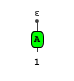
\includegraphics[scale=0.99]{obrazky/sxsx1.png}
}
\qquad
\subfloat[$T(2)$.]{
\label{img:sxsx2}
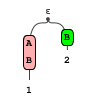
\includegraphics[scale=0.99]{obrazky/sxsx2.png}
}
\qquad
\subfloat[$T(3)$.]{
\label{img:sxsx3}
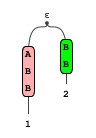
\includegraphics[scale=0.99]{obrazky/sxsx3.png}
}
% \qquad

\subfloat[$T(4)$.]{
\label{img:sxsx4}
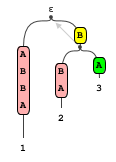
\includegraphics[scale=0.99]{obrazky/sxsx4.png}
}
\qquad
\subfloat[$T$.]{
\label{img:sxsx5}
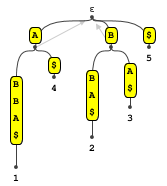
\includegraphics[scale=0.99]{obrazky/sxsx5.png}
}
\caption{\emph{Sufixové stromy.} Na obrázku sú sufixové stromy pre slová 
{\tt A}, {\tt AB}, {\tt ABB}, {\tt ABBA}, {\tt ABBA\uz}. Šípky znázorňujú 
sufixové linky, ružovou a zelenou sú označené hrany, na ktoré sa bude v 
nasledujúcom, kroku aplikovať prvé pravidlo. Čísla oznažujú, na ktorom znaku 
začína daný sufix v slove.}
\label{img:sxsx}
\end{figure}

\subsection{Zhrnutie}

Sufixový strom $T$ pre slovo $w = w_1w_2w_3\cdots w_n\uz$ vytvoríme tak, že z 
prázdneho stromu vytvoríme postupne stromy $T(1), T(2), T(3),\ldots, T(n), 
T(n+1) = T$. 

Strom $T(1)$ vytvoríme triviálne; pridáme koreňu hranu s dvojicou indexov 
$(1, e)$ a nastavíme štartovací vrchol $u_s$ na práve vytvorený vrchol.

Postupne vytvárame strom $T(i)$ zo stromu $T(i-1)$ rozšírením stromu 
$T(i-1)$ o písmenko $w_i$ následovne:

\begin{enumerate}
\item index $e$ nastavíme na novú hodnotu $i$; 
Tým sme vykonali všetky prvé prípady. Vieme si udržiavať ich počet $j$;
\item za aktuálny vrchol $u$ si zvolíme štartovací vrchol $u_s$;
\item z aktuálneho vrcholu prejdeme po hrane vyššie a zapamätáme si reťazec 
na hrane po ktorej sme prešli;
\item ak nie sme v koreni, prejdeme po sufixovom linku. Nastavíme aktuálny 
vrchol;
\item z aktuálneho vrcholu vyhľadáme reťazec $w_{j+1}\cdots w_i$;
\item teraz môže nastať druhý alebo tretí prípad:
\begin{itemize}
\item ak nastal druhý prípad, v prípade potreby rozdelíme hranu. Nastavíme 
aktuálny vrchol na posledný navštívený (respektíve vytvorený) a v prípade 
potreby nastavíme sufixový link. K aktívnemu vrcholu pripojíme hranu s 
indexami $(i,e)$, zvýšime index $j$ o 1 a nastavíme štartovací vrchol na 
práve vytvorený. Vrátime sa na krok~3;
\item ak nastal tretí prípad, v prípade potreby nastavíme sufixový link.
\end{itemize}
\item zvýšime hodnotu $i$ o jeden a vrátime sa na krok 1.
\end{enumerate}
 
Takto vybudujeme sufixový strom pre slovo $w$.

\section{Použitie}\label{sec:sx:usage}

Sufixový strom má v stringológií veľa využití \citep{gusfield}. Algoritmus na 
zistenie prítomnosti podreťazca v slove je rovnaký ako pri písmenkovom strome. 
Navyše vieme určiť, na ktorej pozícií sa podreťazec vyskytuje. Pri 
konštrukcii stromu stačí označovať listy číslami v poradí podľa vytvorenia. 
Hľadanie podreťazca~$p$ v predspracovanom texte~$T$ nám zaberie len 
$O(|p|)$~krokov.

Sufixový strom pre viacej reťazcov sa nazýva \emph{všeobecný sufixový strom} 
a dá sa zostrojiť miernou úpravou Ukkonenovho algoritmu. Reťazce $v_1, v_2, 
v_3, \ldots, v_n$ spojíme a oddelíme unikátnymi oddelovačmi. Vznikne nám slovo 
$v_1\uz_1v_2\uz_2v_3\uz_3\cdots v_n\uz_n$, z ktorého vieme vybudovať sufixový 
strom. Tento strom sa dá využiť na vyhľadanie \emph{najdlhšieho spoločného 
podreťazca}. 

\emph{Najdlhší opakujúci sa podreťazec} sa v sufixovom strom určite vetví, 
takže ho nájdeme ako najdlhšie podslovo, ktoré sa nekončí v liste.

Pre slovo $\alpha$ vieme pomocou sufixových stromov nájsť efektívne 
\emph{najdlhšie palindormatické podslovo}, čo je slovo $\beta \subset \alpha$ 
také, že $\beta^R = \beta$. Zostrojíme všeobecný sufixový strom pre slová 
$\beta$ a $\beta^R$. Pre tento strom vieme efektívne zostrojiť dátovú 
štruktúru pre najnižšieho spoločného predka \citep{lca}. Potom nám stačí 
pre každý index $q$ od $1$ po $n-1$ hľadať najnižšieho spoločného predka pre 
sufixy $w[q:n]$ a $w^R[n-q:n]$.

% \section{Vizualizácia}
% 
% Sufixový strom sme vizualizovali podobne ako písmenkový strom, použili sme 
% Walkerov algoritmus \citep{walker} so zakrivenými hranami. Sufixové linky 
% sme znázornili šedými šípkami. Na rozdiel od písmenkového stromu sa v 
% sufixovom strome vyskytujú na hranách reťazce. Tie sme znázornili ako viac 
% spojených hrán.
% 
% Pri vizualizácií algoritmu oznažujeme hrany, pre ktoré platí prvý prípad, 
% ružovou farbou. Hranu, pre ktorú platí prvý prípad a je pridaná ako posledná, 
% označujeme zelenou farbou. Z tejto hrany začína "zaujímavejšia" časť 
% rozširovania stromu.


